\chapter{Pedestal Modeling and Theory}\label{ch:Modeling}

While a number of high-performance regimes (described in \cref{ch:HighPerformance}) have been established and are actively explored for tokamak operation, much of the physics governing these regimes is still unknown.  In particular, the physics underlying the structure of the pedestal is an area of active research, due in large part to the inherent difficulty in experimentally diagnosing the pedestal plasma as it varies over short scale lengths, and in the wide variability of H-mode behaviors observed in tokamak experiments.  Nevertheless confidence in the prediction of pedestal height and stability for ITER- and reactor-scale devices is essential: core temperature and pressure in the plasma are strongly sensitive to pedestal conditions due to profile stiffness driven by marginally-stable temperature-gradient modes \cite{Hubbard1998}\gnote{elaborate or reword}, thus fusion power density is controlled by the pressure pedestal structure.  Moreover, operation with large, uncontrolled Edge-Localized Modes (ELMs -
- see \cref{sec:hcr_elmy}) can drive transient heat loads exceeding wall material tolerances on ITER-scale devices \cite{Loarte2003,Federici2003} -- an understanding of pedestal stability against ELMs is necessary for ITER operation and beyond.  This chapter provides a review of the efforts to date in theory and modeling of the pedestal, including the theoretical models used in the balance of this thesis.\nicesectionending\gnote{elaborate?}

\section{Early Models}\label{sec:mod_early}

\gnote{needs better title...}Initial efforts in understanding the pedestal took a variety of approaches, including models built from fairly simple \emph{ans\:atze} for the physics determining the pedestal structure.  Several of these approaches are detailed here.  Overviews of these models may also be found in \cite[\S 2]{Hubbard2000,Hughes2005}.

\subsection{Neutral Penetration \& the Density Pedestal}\label{subsec:mod_neutral}

Given the proximity of the plasma pedestal to neutral gas from fueling apparatus and wall outgassing in the edge, it is logical that the density profile should depend strongly on interaction with and ionization of neutral particles in the pedestal.  Based on a relatively simple particle transport model, the pedestal width is expected to scale with the characteristic neutral penetration length before ionization \cite{Hughes2005,Mahdavi2002}:

\begin{equation}\label{eq:neutralpenetration}
 \lambda_{neutral} = \frac{v_n}{n_e \langle \sigma v \rangle_{ion}}
\end{equation}

\noindent where $v_n$ is the velocity of neutrals entering the pedestal (set by the neutral thermal temperature in the edge) and $\langle \sigma v \rangle_{ion}$ is the velocity-averaged ionization cross-section.  Given that $v_n$ is independent of plasma conditions and that $\langle \sigma v \rangle_{ion}$ is consistent over the temperatures of interest in the edge \cite{Hughes2005}, therefore we expect the simple relation $\Delta_{n} \sim 1/n_{e,ped}$.  More complex models for the neutral penetration typically reproduce the dependence on $\lambda_{neutral}$.

However, experimental observations of the density pedestal conflict with these relatively simple predictions.    Observations in similarity experiments between DIII-D, JET, and ASDEX Upgrade \cite{Beurskens2011} were inconsistent with the simple model: although DIII-D data were consistent with the trends found in the model, data from JET were not, and moreover the model predicted an inconsistent scaling between the two machines for pedestal density and width.  Likewise, predictions based on pedestal widths set by neutral penetration performed poorly as a predictor for pedestal height in a multi-machine scaling from AUG, DIII-D, JT-60U, and JET \cite{Onjun2002}.  EDA H-modes on Alcator C-Mod show near-complete insensitivity of the density pedestal to neutral interactions -- the density pedestal instead saturates to a level dictated by plasma transport (predicted best by $n_{e,ped} \sim I_p$), with fueling via edge gas puffing having little effect on the density pedestal \cite{Hughes2006,Hughes2007}.

In addition to significant sensitivity to machine and discharge conditions and wall materials \cite{Beurskens2011}, density pedestal behavior appears to be strongly sensitive to magnetic configuration -- experiments on MAST \cite{Maggi2010} found that, while the density pedestal width was poloidally constant in single-null discharges, the density pedestal is measurably broader on the outboard, low-field side in double-null discharges.  These results indicate that plasma-neutral interactions in the density pedestal are quite complex, and dependent on poloidal transport behaviors and fueling asymmetries \cite{Maggi2010}.  This remains an important area of research, as ITER is expected to have an edge that is highly opaque to neutrals, complicating the density pedestal structure and fueling scenarios for high-density plasmas \cite{Hughes2007,Maggi2010}.

\subsection{Ion-Orbit Loss \& Gyroradius Models}\label{subsec:mod_ionorbitloss}

Due to the importance in the edge $E_r$ well in pedestal formation, modeling efforts naturally turned to potential sources for the electric field to explain the pedestal.  One suggested source was ion orbit loss across the last closed flux surface, in which the gyro-motion of ions near the edge intersect the SOL or the plasma-facing material surfaces -- the charge imbalance induced by this particle ``leak'' results in a radial electric field \cite{Shaing1990}.  Assuming ion orbit losses drive the $E_r$ well, the $\vec{E}\times\vec{B}$ shear layer width ought to be governed by the banana orbit width, which scales as the poloidal gyroradius $\rho_{i,pol} \sim \sqrt{T_i}/B_p$.  Accounting for the squeezing effect of the radial electric field on the banana orbit width, Shaing \cite{Shaing1992} gives for the well width

\begin{equation}\label{eq:Shaing_width}
 \begin{aligned}
  &\Delta_{\vec{E}\times\vec{B}} \propto \sqrt{\varepsilon} \frac{\rho_{i,pol}}{\sqrt{S}}\\
  &S = \left| 1 - \frac{1}{B_p \omega_{ci,p}} \frac{dE_r}{dr}\right|
 \end{aligned}
\end{equation}

\noindent where $S$ is the squeezing factor and $\omega_{ci,p}$ is the ion cyclotron frequency evaluated with the poloidal field.  The model is further refined by Itoh \& Itoh \cite{Itoh1996} to include the broadening effects of viscosity shear.  The predicted trend is observed in ELM-free H-modes on JT-60U \cite{Hatae1998}, with $\Delta \approx 3.3 \sqrt{\varepsilon} \rho_{i,pol}$; however, as the squeezing factor $S$ is estimated to be near-unity, the pedestal width is broader by a factor of $\sim 3.3$ than the $\sim \sqrt{\varepsilon} \rho_{i,pol}$ banana width.  ELMy H-modes on JT-60U exhibit a similar scaling at weak shaping, with a broader pedestal and additional safety factor dependence $\Delta \approx 5 \rho_{i,pol} q_{95}^{-0.3}$ at higher triangularity \cite{Kamada1999}.

However, observations on other machines contradict these results.  Depending on the calculation method of growth rate suppression by $\vec{E}\times\vec{B}$ sheared flow, the pedestal width may scale with the gyroradius anywhere from $\Delta \sim \left(\rho^*\right)^{1/2}$ to $\Delta \sim \rho^*$, where $\rho^*$ indicates the gyroradius normalized to the plasma minor radius \cite{Beurskens2011}.  Distinguishing between these scalings is difficult given the diagnostic complications inherent in pedestal measurements, and the narrow range over which $\rho^*$ or the pedestal and $E_r$ well width vary on a given machine\gnote{cite or elaborate - Gohil cite?}.

\subsection{Empirical Observations}\label{subsec:mod_empirical}

\nicesectionending

\section{MHD Stability: Peeling-Ballooning Modes}\label{sec:mod_pb}

\subsection{Ballooning MHD}\label{subsec:mod_balloon}

\subsection{Peeling MHD}\label{subsec:mod_peel}

\subsection{ELITE Code}\label{subsec:mod_elite}

\begin{figure}
 \pushtooutside
 \fcapside[60mm]{\caption{Schematic of the stability space to coupled peeling-ballooning MHD modes, set by the edge pressure gradient and current density.  Ballooning modes are driven by pressure gradient but stabilized by magnetic shear driven by edge currents, while kink/peeling modes are current-driven but stabilized by pressure gradients.  \note{Ref to Snyder?}}\label{fig:mod_pbcartoon}}{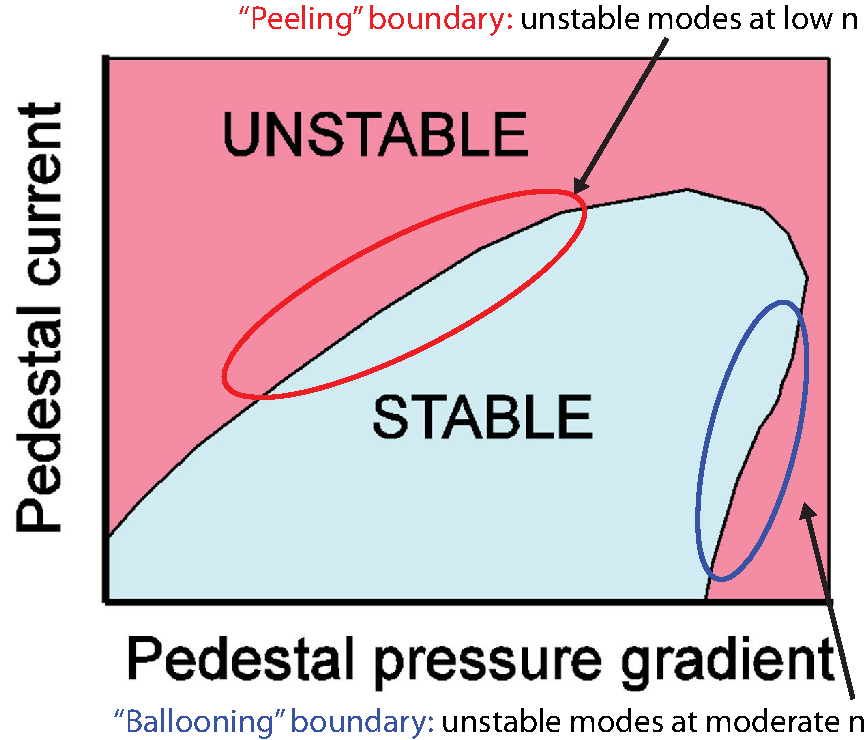
\includegraphics[width=100mm]{graphics/ModelingTheory/pbcartoon.pdf}}
\end{figure}

\nicesectionending

\section{Turbulent Modeling}\label{sec:mod_turbulence}

\nicesectionending

\section{The EPED Model}\label{sec:mod_eped}

\begin{figure}
 \pushtooutside
 \fcapside[60mm]{\caption{EPED predictions versus measured pressure pedestal heights from DIII-D and C-Mod, spanning a significant range of pedestal pressures.  Notably, C-Mod pressure pedestals reach within a factor of $\sim 2$ of the predicted ITER pedestal height.  \note{ref to Hughes paper}}\label{fig:mod_epedpredictions}}{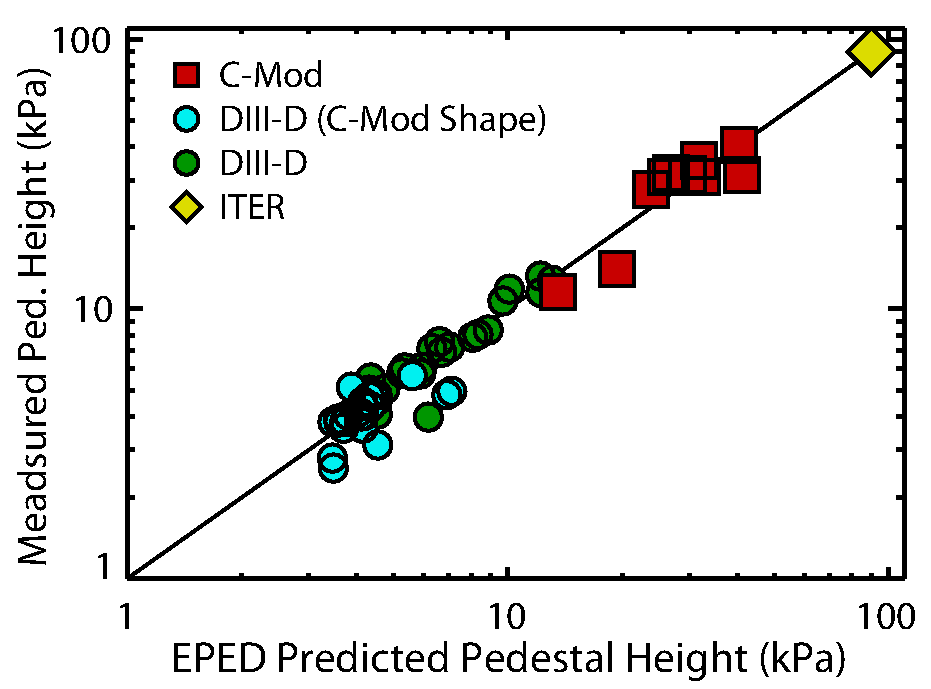
\includegraphics[width=100mm]{graphics/ModelingTheory/eped.pdf}}
\end{figure}


\nicechapterending

\bibliographystyle{../plainurl}
\bibliography{../references}